
\appendix
\section{Appendix}


\subsection{Robustness}
\label{sec:robust}

\begin{figure}[H]
	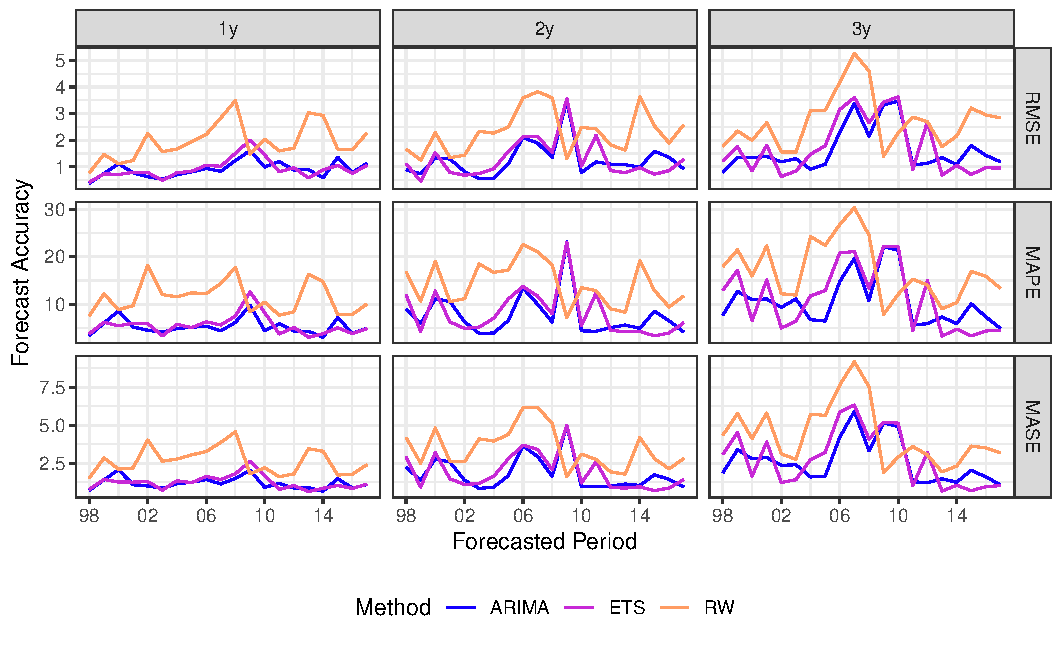
\includegraphics[width=\textwidth]{fig/fig_eval_methods_top}
	\caption{Accuracy of Forecasting Methods at the Top Level}
\end{figure}

\begin{figure}[H]
	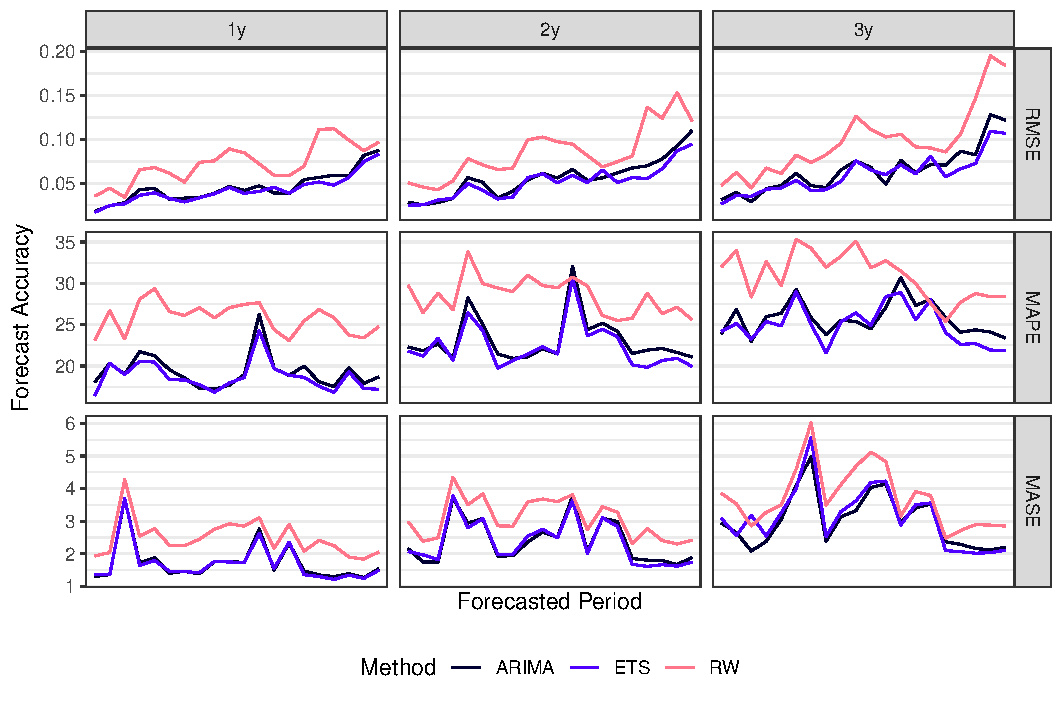
\includegraphics[width=\textwidth]{fig/fig_eval_methods_bottom}
	\caption{Accuracy of Forecasting Methods at the Bottom Level}
\end{figure}


\subsection{Data}
\label{sec:data}
The data is compiled by the Swiss Federal Customs Administration\footnote{\url{https://www.ezv.admin.ch/ezv/en/home/topics/swiss-foreign-trade-statistics.html}}.\\

\begin{small}
\begin{longtable}{p{2.5cm}p{11.5cm}}
\caption{Description of Categorical Hierarchy}\\
\toprule
\normalsize{Tariff Number} & \normalsize{Description}\\
\midrule
\endfirsthead
\multicolumn{2}{@{}l}{\ldots continued}\\
\toprule
\normalsize{Tariff Number} & \normalsize{Description}\\  
\midrule
\endhead
\bottomrule
\multicolumn{2}{r@{}}{continued \ldots}\\
\endfoot
\bottomrule
\endlastfoot
	01	&	Forestry and agricultural products, fisheries	\\
\enskip	01.1	&	Food, beverages and tobacco	\\
\enskip	01.2	&	Feeding stuffs for animals	\\
\enskip	01.3	&	Live animals	\\
\enskip	01.4	&	Horticultural products	\\
\enskip	01.5	&	Forestry products (not firewood)	\\
\enskip	01.6	&	Products for commercial/industrial further processing such as oils, fats, starches, plants and vegetable parts, etc.	\\
\midrule
	02	&	Energy source	\\
\enskip	02.1	&	Solid combustibles	\\
\enskip	02.2	&	Petroleum and distillates	\\
\enskip	02.3	&	Gas	\\
\enskip	02.4	&	Electrical energy	\\
\midrule
	03	&	Textiles, clothing, shoes	\\
\enskip	03.1	&	Textiles	\\
\enskip	03.2	&	Articles of apparel and clothing	\\
\enskip	03.3	&	Shoes, parts and accessories	\\
\midrule
	04	&	Paper, articles of paper and and products of the printing industry	\\
\enskip	04.1	&	Basic materials for paper production, such as cellulose and cellulose fibre and paper and carton waste	\\
\enskip	04.2	&	Paper and carton in rolls, strips or sheets	\\
\enskip	04.3	&	Goods from paper or carton	\\
\enskip	04.4	&	Products of the printing industry	\\
\midrule
	05	&	Leather, rubber, plastics	\\
\enskip	05.1	&	Leather	\\
\enskip	05.2	&	Rubber	\\
\enskip	05.3	&	Plastics	\\
\midrule
	06	&	Products of the chemical and pharmaceutical industry	\\
\enskip	06.1	&	Chemical raw materials, basic materials and unformed plastics	\\
\enskip	06.2	&	Chemical end products, vitamins, diagnostic products, including active substances	\\
\midrule
	07	&	Stones and earth	\\
\enskip	07.1	&	Mineral raw materials and basic products	\\
\enskip	07.2	&	Goods from stone and cement	\\
\enskip	07.3	&	Ceramic wares	\\
\enskip	07.4	&	Glass	\\
\midrule
	08	&	Metals	\\
\enskip	08.1	&	Iron and steel	\\
\enskip	08.2	&	Non-ferrous metals	\\
\enskip	08.3	&	Metal goods	\\
\midrule
	09	&	Machines, appliances, electronics	\\
\enskip	09.1	&	Industrial machinery	\\
\enskip	09.2	&	Agricultural machines	\\
\enskip	09.3	&	Household appliances	\\
\enskip	09.4	&	Office machines	\\
\enskip	09.5	&	Electrical and electronic industry appliances and devices	\\
\enskip	09.6	&	Military equipment	\\
\midrule
	10	&	Vehicles	\\
\enskip	10.1	&	Road vehicles	\\
\enskip	10.2	&	Railed vehicles	\\
\enskip	10.3	&	Air- and spacecraft	\\
\enskip	10.4	&	Watercraft	\\
\midrule
	11	&	Precision instruments, clocks and watches and jewellery	\\
\enskip	11.1	&	Precision instruments and equipment	\\
\enskip	11.2	&	Watches	\\
\enskip	11.3	&	Jewellery and household goods made from precious metals	\\
\midrule
	12	&	Various goods such as music instruments, home furnishings, toys, sports equipment, etc.	\\
\enskip	12.1	&	Exposed film	\\
\enskip	12.2	&	Music instruments	\\
\enskip	12.3	&	Home furnishings	\\
\enskip	12.4	&	Toys and sports equipment	\\
\enskip	12.5	&	Stationery goods	\\
\enskip	12.6	&	Various goods such as umbrellas, neon signs, festive articles, brushes, lighters, pipes, etc.	\\
\midrule
	13	&	Precious metals, precious and semi-precious stones	\\
\enskip	13.1	&	Precious and semi-precious stones	\\
\enskip	13.2	&	Precious metals (including gold and silver bars from 1.1.2012)	\\
\midrule
	14	&	Works of art and antiques	\\
\enskip	14.1	&	Works of art	\\
\enskip	14.2	&	Antiques and collectors' items	\\
\end{longtable}
\end{small}

\clearpage

\begin{small}
	\begin{longtable}{p{7.5cm}cccc}
		\caption{Description of Geographical Hierarchy}\\
		\toprule
Country	&	isoCode	&	regCode	&	valid from	&	valid to	\\
		\midrule
		\endfirsthead
		\multicolumn{4}{@{}l}{\ldots continued}\\
		\toprule
Country	&	isoCode	&	regCode	&	valid from	&	valid to	\\
		\midrule
		\endhead
		\bottomrule
		\multicolumn{4}{r@{}}{continued \ldots}\\
		\endfoot
		\bottomrule
		\endlastfoot
Switzerland	&	CH	&	EU	&	01/1988	&	-	\\
Germany	&	DE	&	EU	&	01/1988	&	-	\\
France	&	FR	&	EU	&	01/1988	&	-	\\
Italy	&	IT	&	EU	&	01/1988	&	-	\\
Netherlands	&	NL	&	EU	&	01/1988	&	-	\\
Belgium-Luxembourg	&	BE	&	EU	&	01/1988	&	12/1998	\\
Belgium	&	BE	&	EU	&	01/1999	&	-	\\
Luxembourg	&	LU	&	EU	&	01/1999	&	-	\\
Austria	&	AT	&	EU	&	01/1988	&	-	\\
United Kingdom	&	GB	&	EU	&	01/1988	&	-	\\
Denmark	&	DK	&	EU	&	01/1988	&	-	\\
Norway	&	NO	&	EU	&	01/1988	&	-	\\
Sweden	&	SE	&	EU	&	01/1988	&	-	\\
Portugal	&	PT	&	EU	&	01/1988	&	-	\\
Finland	&	FI	&	EU	&	01/1988	&	-	\\
Croatia, Republic of	&	HR	&	EU	&	02/1992	&	-	\\
Slovenia	&	SI	&	EU	&	02/1992	&	-	\\
Bosnia and Herzegovina	&	BA	&	EU	&	05/1992	&	-	\\
Macedonia	&	MK	&	EU	&	05/1992	&	-	\\
Montenegro	&	ME	&	EU	&	05/1992	&	12/1996	\\
Montenegro	&	ME	&	EU	&	01/2007	&	-	\\
Montenegro	&	XM	&	EU	&	01/2006	&	12/2006	\\
Serbia	&	SQ	&	EU	&	05/1992	&	12/1996	\\
Serbia	&	RS	&	EU	&	01/2007	&	-	\\
Serbia	&	XS	&	EU	&	01/2006	&	12/2006	\\
Federal Republic of Yugoslavia	&	YU	&	EU	&	01/1997	&	12/2003	\\
Serbia and Montenegro	&	CS	&	EU	&	01/2004	&	12/2005	\\
Kosovo	&	XK	&	EU	&	01/2006	&	-	\\
Iceland	&	IS	&	EU	&	01/1988	&	-	\\
Ireland	&	IE	&	EU	&	01/1988	&	-	\\
Spain	&	ES	&	EU	&	01/1988	&	-	\\
Greece	&	GR	&	EU	&	01/1988	&	-	\\
Turkey	&	TR	&	EU	&	01/1988	&	-	\\
GDR	&	DD	&	EU	&	01/1988	&	10/1990	\\
Poland	&	PL	&	EU	&	01/1988	&	-	\\
Czech Republic	&	CZ	&	EU	&	01/1993	&	-	\\
Czechoslovakia	&	CS	&	EU	&	01/1988	&	02/1992	\\
Slovakia	&	SK	&	EU	&	01/1993	&	-	\\
Hungary	&	HU	&	EU	&	01/1988	&	-	\\
Albania	&	AL	&	EU	&	01/1988	&	-	\\
Bulgaria, Republic of	&	BG	&	EU	&	01/1988	&	-	\\
Romania	&	RO	&	EU	&	01/1988	&	-	\\
USSR	&	SU	&	EU	&	01/1988	&	12/1991	\\
Yugoslavia	&	YU	&	EU	&	01/1988	&	04/1992	\\
Cyprus	&	CY	&	EU	&	01/1988	&	-	\\
Svalbard and Jan Mayen Island	&	SJ	&	EU	&	01/1999	&	-	\\
Malta	&	MT	&	EU	&	01/1988	&	-	\\
Gibraltar	&	GI	&	EU	&	01/1988	&	-	\\
Faeroe Islands	&	FO	&	EU	&	01/1988	&	-	\\
San Marino	&	SM	&	EU	&	01/1999	&	-	\\
Holy See	&	VA	&	EU	&	01/1999	&	-	\\
Andorra	&	AD	&	EU	&	01/1988	&	-	\\
Estonia	&	EE	&	EU	&	01/1992	&	-	\\
Latvia	&	LV	&	EU	&	01/1992	&	-	\\
Lithuania	&	LT	&	EU	&	01/1992	&	-	\\
Russian Federation	&	RU	&	CA	&	01/1992	&	-	\\
Armenia	&	AM	&	CA	&	01/1992	&	-	\\
Azerbaijan	&	AZ	&	CA	&	01/1992	&	-	\\
Belarus	&	BY	&	CA	&	01/1992	&	-	\\
Georgia	&	GE	&	CA	&	01/1992	&	-	\\
Kazakhstan	&	KZ	&	CA	&	01/1992	&	-	\\
Kyrgyz, Republic	&	KG	&	CA	&	01/1992	&	-	\\
Moldova, Republic of	&	MD	&	CA	&	01/1992	&	-	\\
Tajikistan	&	TJ	&	CA	&	01/1992	&	-	\\
Turkmenistan	&	TM	&	CA	&	01/1992	&	-	\\
Ukraine	&	UA	&	CA	&	01/1992	&	-	\\
Uzbekistan	&	UZ	&	CA	&	01/1992	&	-	\\
Egypt	&	EG	&	AF	&	01/1988	&	-	\\
Sudan	&	SD	&	AF	&	01/1988	&	-	\\
South Sudan, Republic of	&	SS	&	AF	&	09/2011	&	-	\\
Libya	&	LY	&	AF	&	01/1988	&	-	\\
Tunisia	&	TN	&	AF	&	01/1988	&	-	\\
Algeria	&	DZ	&	AF	&	01/1988	&	-	\\
Canary Islands	&	XA	&	AF	&	01/1988	&	-	\\
Morocco	&	MA	&	AF	&	01/1988	&	-	\\
Western Sahara	&	EH	&	AF	&	01/1999	&	-	\\
Ceuta and Melilla	&	XB	&	AF	&	01/1988	&	12/2010	\\
Equatorial Guinea	&	GQ	&	AF	&	01/1988	&	-	\\
Ceuta	&	XC	&	AF	&	01/2001	&	-	\\
Melilla	&	XL	&	AF	&	01/2001	&	-	\\
Togo	&	TG	&	AF	&	01/1988	&	-	\\
Senegal	&	SN	&	AF	&	01/1988	&	-	\\
Mali	&	ML	&	AF	&	01/1988	&	-	\\
Mauritania	&	MR	&	AF	&	01/1988	&	-	\\
Côte d'Ivoire	&	CI	&	AF	&	01/1988	&	-	\\
Burkina Faso	&	BF	&	AF	&	01/1988	&	-	\\
Benin	&	BJ	&	AF	&	01/1988	&	-	\\
Niger	&	NE	&	AF	&	01/1988	&	-	\\
Guinea	&	GN	&	AF	&	01/1988	&	-	\\
Gambia	&	GM	&	AF	&	01/1988	&	-	\\
Sierra Leone	&	SL	&	AF	&	01/1988	&	-	\\
Liberia	&	LR	&	AF	&	01/1988	&	-	\\
Ghana	&	GH	&	AF	&	01/1988	&	-	\\
Nigeria, Federal Republic of	&	NG	&	AF	&	01/1988	&	-	\\
Cameroon	&	CM	&	AF	&	01/1988	&	-	\\
Gabon	&	GA	&	AF	&	01/1988	&	-	\\
Congo, Republic of the	&	CG	&	AF	&	01/1988	&	-	\\
Central African Republic	&	CF	&	AF	&	01/1988	&	-	\\
Chad	&	TD	&	AF	&	01/1988	&	-	\\
Congo, Democratic Republic of the	&	CD	&	AF	&	06/1997	&	-	\\
Zaire	&	ZR	&	AF	&	01/1988	&	05/1997	\\
Angola	&	AO	&	AF	&	01/1988	&	-	\\
Guinea-Bissau	&	GW	&	AF	&	01/1988	&	-	\\
Botswana	&	BW	&	AF	&	01/1988	&	-	\\
Cabo Verde, Republic of	&	CV	&	AF	&	01/1988	&	-	\\
Lesotho	&	LS	&	AF	&	01/1988	&	-	\\
Sao Tomé and Principe	&	ST	&	AF	&	01/1988	&	-	\\
Namibia	&	NA	&	AF	&	01/1988	&	-	\\
South Africa	&	ZA	&	AF	&	01/1988	&	-	\\
Swaziland	&	SZ	&	AF	&	01/1988	&	-	\\
Zambia	&	ZM	&	AF	&	01/1988	&	-	\\
Zimbabwe	&	ZW	&	AF	&	01/1988	&	-	\\
Malawi	&	MW	&	AF	&	01/1988	&	-	\\
Mozambique	&	MZ	&	AF	&	01/1988	&	-	\\
Madagascar, Republic of	&	MG	&	AF	&	01/1988	&	-	\\
Réunion	&	RE	&	AF	&	01/1988	&	-	\\
St Helena, Ascen. and Tristan da Cunha	&	SH	&	AF	&	01/1988	&	-	\\
Comoros, Union of	&	KM	&	AF	&	01/1988	&	-	\\
Antarctica	&	AQ	&	AF	&	01/1988	&	-	\\
Mauritius	&	MU	&	AF	&	01/1988	&	-	\\
British Indian Ocean Territory	&	IO	&	AF	&	01/1988	&	-	\\
Tanzania, United Republic of	&	TZ	&	AF	&	01/1988	&	-	\\
Seychelles, Republic of	&	SC	&	AF	&	01/1988	&	-	\\
Rwanda	&	RW	&	AF	&	01/1988	&	-	\\
Bouvet Island	&	BV	&	AF	&	01/1999	&	-	\\
Burundi	&	BI	&	AF	&	01/1988	&	-	\\
Mayotte	&	YT	&	AF	&	01/1999	&	-	\\
Somalia, Federal Republic of	&	SO	&	AF	&	01/1988	&	-	\\
French Southern Territories	&	TF	&	AF	&	01/1999	&	-	\\
Djibouti	&	DJ	&	AF	&	01/1988	&	-	\\
Eritrea	&	ER	&	AF	&	01/1994	&	-	\\
Ethiopia, Fed. Democratic Republic of	&	ET	&	AF	&	01/1988	&	-	\\
Kenya	&	KE	&	AF	&	01/1988	&	-	\\
Uganda	&	UG	&	AF	&	01/1988	&	-	\\
Syrian Arab Republic	&	SY	&	AF	&	01/1988	&	-	\\
Lebanon	&	LB	&	AF	&	01/1988	&	-	\\
Israel	&	IL	&	AF	&	01/1988	&	-	\\
Palestine, the State of	&	PS	&	AF	&	01/1997	&	-	\\
Jordan	&	JO	&	AF	&	01/1988	&	-	\\
Saudi Arabia	&	SA	&	AF	&	01/1988	&	-	\\
Yemen (Nord)	&	YE	&	AF	&	01/1988	&	12/1990	\\
Yemen	&	YE	&	AF	&	01/1991	&	-	\\
Yemen (Sud)	&	YD	&	AF	&	01/1988	&	12/1990	\\
Qatar	&	QA	&	AF	&	01/1988	&	-	\\
Bahrain	&	BH	&	AF	&	01/1988	&	-	\\
United Arab Emirates	&	AE	&	AF	&	01/1988	&	-	\\
Oman	&	OM	&	AF	&	01/1988	&	-	\\
Kuwait	&	KW	&	AF	&	01/1988	&	-	\\
Iraq	&	IQ	&	AF	&	01/1988	&	-	\\
Iran, Islamic Republic of	&	IR	&	AF	&	01/1988	&	-	\\
Afghanistan	&	AF	&	SA	&	01/1988	&	-	\\
Pakistan	&	PK	&	SA	&	01/1988	&	-	\\
Bangladesh	&	BD	&	SA	&	01/1988	&	-	\\
India	&	IN	&	SA	&	01/1988	&	-	\\
Sri Lanka	&	LK	&	SA	&	01/1988	&	-	\\
Maldives	&	MV	&	SA	&	01/1988	&	-	\\
Nepal, Federal Democratic Rep.	&	NP	&	SA	&	01/1988	&	-	\\
Bhutan	&	BT	&	SA	&	01/1988	&	-	\\
Myanmar, Union of	&	MM	&	EA	&	01/1988	&	-	\\
Thailand	&	TH	&	EA	&	01/1988	&	-	\\
Malaysia	&	MY	&	EA	&	01/1988	&	-	\\
Brunei Darussalam	&	BN	&	EA	&	01/1988	&	-	\\
Singapore	&	SG	&	EA	&	01/1988	&	-	\\
Cambodia	&	KH	&	EA	&	01/1988	&	-	\\
Lao, People's Democratic Republic	&	LA	&	EA	&	01/1988	&	-	\\
Viet Nam, Socialist Republic of	&	VN	&	EA	&	01/1988	&	-	\\
Mongolia	&	MN	&	EA	&	01/1988	&	-	\\
China, People's Republic of	&	CN	&	EA	&	01/1988	&	-	\\
Hong Kong	&	HK	&	EA	&	01/1988	&	-	\\
Taiwan	&	TW	&	EA	&	01/1988	&	-	\\
Macau	&	MO	&	EA	&	01/1988	&	-	\\
Korea, People's Democratic Republic of	&	KP	&	EA	&	01/1988	&	-	\\
Korea, Republic of	&	KR	&	EA	&	01/1988	&	-	\\
Japan	&	JP	&	EA	&	01/1988	&	-	\\
Philippines	&	PH	&	EA	&	01/1988	&	-	\\
Indonesia	&	ID	&	EA	&	01/1988	&	-	\\
East Timor	&	TL	&	EA	&	01/2004	&	-	\\
East Timor	&	TP	&	EA	&	01/1999	&	12/2003	\\
Canada	&	CA	&	NA	&	01/1988	&	-	\\
St Pierre and Miquelon	&	PM	&	NA	&	01/1988	&	-	\\
United States	&	US	&	NA	&	01/1988	&	-	\\
Greenland	&	GL	&	NA	&	01/1988	&	-	\\
Mexico	&	MX	&	LA	&	01/1988	&	-	\\
Belize	&	BZ	&	LA	&	01/1988	&	-	\\
Guatemala	&	GT	&	LA	&	01/1988	&	-	\\
Honduras	&	HN	&	LA	&	01/1988	&	-	\\
El Salvador	&	SV	&	LA	&	01/1988	&	-	\\
Nicaragua	&	NI	&	LA	&	01/1988	&	-	\\
Costa Rica	&	CR	&	LA	&	01/1988	&	-	\\
Panama	&	PA	&	LA	&	01/1988	&	-	\\
Cayman Islands	&	KY	&	LA	&	01/1988	&	-	\\
Turks and Caicos Islands	&	TC	&	LA	&	01/1988	&	-	\\
Bahamas	&	BS	&	LA	&	01/1988	&	-	\\
Bermuda	&	BM	&	LA	&	01/1988	&	-	\\
Jamaica	&	JM	&	LA	&	01/1988	&	-	\\
Cuba	&	CU	&	LA	&	01/1988	&	-	\\
Haiti	&	HT	&	LA	&	01/1988	&	-	\\
Dominican Republic	&	DO	&	LA	&	01/1988	&	-	\\
American Virgin Islands	&	VI	&	LA	&	01/1988	&	-	\\
Puerto Rico	&	PR	&	LA	&	01/1988	&	12/2005	\\
Dominica	&	DM	&	LA	&	01/1988	&	-	\\
St Vincent and the Grenadines	&	VC	&	LA	&	01/1988	&	-	\\
St Lucia	&	LC	&	LA	&	01/1988	&	-	\\
Montserrat	&	MS	&	LA	&	01/1988	&	-	\\
Antigua and Barbuda	&	AG	&	LA	&	01/1988	&	-	\\
Barbados	&	BB	&	LA	&	01/1988	&	-	\\
Grenada	&	GD	&	LA	&	01/1988	&	-	\\
St Kitts and Nevis	&	KN	&	LA	&	01/1988	&	-	\\
Anguilla	&	AI	&	LA	&	01/1988	&	-	\\
Guadeloupe	&	GP	&	LA	&	01/1988	&	-	\\
British Virgin Islands	&	VG	&	LA	&	01/1999	&	-	\\
Martinique	&	MQ	&	LA	&	01/1988	&	-	\\
Trinidad and Tobago	&	TT	&	LA	&	01/1988	&	-	\\
Saint BarthÈlemy	&	BL	&	LA	&	01/2013	&	-	\\
Netherlands Antilles	&	AN	&	LA	&	01/1988	&	12/2012	\\
Aruba	&	AW	&	LA	&	01/1999	&	-	\\
Bonaire, Sint Eustatius and Saba	&	BQ	&	LA	&	01/2013	&	-	\\
Curacao	&	CW	&	LA	&	01/2013	&	-	\\
Sint Maarten (NL)	&	SX	&	LA	&	01/2013	&	-	\\
Colombia	&	CO	&	LA	&	01/1988	&	-	\\
Venezuela, the Bolivarian Republic of	&	VE	&	LA	&	01/1988	&	-	\\
Guyana	&	GY	&	LA	&	01/1988	&	-	\\
Suriname	&	SR	&	LA	&	01/1988	&	-	\\
French Guiana	&	GF	&	LA	&	01/1988	&	-	\\
Brazil	&	BR	&	LA	&	01/1988	&	-	\\
Paraguay	&	PY	&	LA	&	01/1988	&	-	\\
Uruguay	&	UY	&	LA	&	01/1988	&	-	\\
Argentina	&	AR	&	LA	&	01/1988	&	-	\\
Falkland Islands	&	FK	&	LA	&	01/1988	&	-	\\
South Georgia and South Sandwich Islands	&	GS	&	LA	&	01/1999	&	-	\\
Chile	&	CL	&	LA	&	01/1988	&	-	\\
Bolivia, the Plurinational State of	&	BO	&	LA	&	01/1988	&	-	\\
Peru	&	PE	&	LA	&	01/1988	&	-	\\
Ecuador	&	EC	&	LA	&	01/1988	&	-	\\
Australia	&	AU	&	AO	&	01/1988	&	-	\\
Papua New Guinea	&	PG	&	AO	&	01/1988	&	-	\\
Cocos (Keeling) Islands	&	CC	&	AO	&	01/1999	&	-	\\
Heard and McDonald Islands	&	HM	&	AO	&	01/1999	&	-	\\
Norfolk Island	&	NF	&	AO	&	01/1999	&	-	\\
Christmas Island	&	CX	&	AO	&	01/1999	&	-	\\
New Zealand	&	NZ	&	AO	&	01/1988	&	-	\\
Cook Islands	&	CK	&	AO	&	01/1998	&	-	\\
Samoa	&	WS	&	AO	&	01/1988	&	-	\\
Niue Island	&	NU	&	AO	&	01/1999	&	-	\\
Kiribati, the Republic of	&	KI	&	AO	&	01/1988	&	-	\\
Tokelau Islands	&	TK	&	AO	&	01/1999	&	-	\\
Tuvalu	&	TV	&	AO	&	01/1988	&	-	\\
Pitcairn Islands	&	PN	&	AO	&	01/1988	&	-	\\
Solomon Islands	&	SB	&	AO	&	01/1988	&	-	\\
French Polynesia	&	PF	&	AO	&	01/1988	&	-	\\
New Caledonia	&	NC	&	AO	&	01/1999	&	-	\\
Wallis and Futuna	&	WF	&	AO	&	01/1999	&	-	\\
American Oceania	&	PU	&	AO	&	01/1988	&	12/1996	\\
American Oceania	&	UM	&	AO	&	01/2006	&	-	\\
American Oceania	&	UM	&	AO	&	01/1997	&	12/2005	\\
Northern Mariana, Islands	&	MP	&	AO	&	01/1997	&	-	\\
Marshall Islands	&	MH	&	AO	&	01/1997	&	-	\\
Micronesia, Federated States of	&	FM	&	AO	&	01/1997	&	-	\\
Palau	&	PW	&	AO	&	01/1997	&	-	\\
Fiji, Republic of	&	FJ	&	AO	&	01/1988	&	-	\\
American Samoa	&	AS	&	AO	&	01/2006	&	-	\\
Guam	&	GU	&	AO	&	01/2006	&	-	\\
Vanuatu	&	VU	&	AO	&	01/1988	&	-	\\
Nauru	&	NR	&	AO	&	01/1988	&	-	\\
Tonga	&	TO	&	AO	&	01/1988	&	-	\\
Countries not specified	&	QX	&	EU	&	01/2002	&	-	\\
\end{longtable}
\end{small}

\subsection{Scaling Methods}
\label{subsec:scaling}
by equation (\ref{eq:scale}).
\begin{align}
	\label{eq:scale}
	|\lambda| &= \lambda_1 \lambda_2 \hdots \lambda_m
	= \prod_{s^- = 1}^{x} \lambda_{s^-}\ \eta^{-\frac{1}{x}}   \prod_{s^+ = x+1}^{m} \lambda_{s^+}\ \eta^{\frac{1}{m-x}} = 1
\end{align}
The $x$ local variance components $\lambda_{s^-}$ are scaled down by a factor $\eta^{\frac{1}{x}}$ and the remaining $(m-x)$ components $\lambda_{s^+}$ are correspondingly scaled up by a factor $\eta^{\frac{1}{m-x}}$. The generalized variance remains at unity irrespective of the scaling factor $\eta$ and the number of series to be scaled down $x$. 
